\phantomsection

\chapter{Post-Exploitation}
\markboth{Post-Exploitation}{}
La fase di \emph{Exploitation} ha portato all'acquisizione della macchina target mediante l'accesso al servizio \emph{SSH}. Nell'ambito della presente fase verranno illustrate le attività di \emph{Post-Exploitation} svolte, trattando, in particolare, la fase di \emph{Privilege Escalation} e quella di \emph{Maintaining Access}. 
\section{Privilege Escalation}
Ottenuto l'accesso all'utente \emph{`auxerre'} è stata studiata una strategia volta ad un'elevazione verticale dei privilegi al fine di ottenere l'accesso all'utente \emph{root}. Nei successivi paragrafi verranno illustrate le metodologie utilizzate per la \emph{privilege escalation}.
\subsection{Armitage}
In maniera analoga a quanto accaduto con la fase di \emph{Exploitation}, ci si è avvalsi dell'utilizzo del tool \emph{Armitage} al fine di individuare un exploit in grado di effettuare \emph{privilege escalation} sulla macchina target. Mediante l'interfaccia di \emph{Armitage} è stato effettuato il \emph{log in} al servizio \emph{SSH} della macchina target, per poi effettuare una scansione degli \emph{exploit} disponibili ed infine eseguirli in \emph{flood} mediante la funzionalità \emph{Hail Mary} già sfruttata in fase di \emph{Exploitation}. Tale operazione ha portato alla creazione di una sessione mediante l'\emph{exploit} \emph{`auxiliary/scanner/ssh/ssh\_login'} che è riuscito a stabilire una connessione \emph{SSH} con la macchina target, presumibilmente sfruttando le credenziali inserite in fase di \emph{log in} dall'interfaccia di \emph{Armitage}. Interagendo con la sessione stabilita, è stato verificato, mediante il comando \emph{`whoami'}, che l'accesso è stato effettuato con l'utente \emph{`auxerre} (figura \ref{fig:armitage_ssh}). Non è stato, dunque, rilevato un \emph{exploit} in grado di effettuare una \emph{privilege escalation}.
\begin{figure}[h]
    \centering
    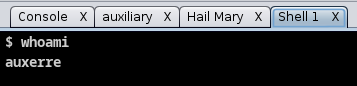
\includegraphics[scale=1]{capitoli/images/armitage_ssh.png}
    \caption{Sessione stabilita da \emph{Armitage}}
    \label{fig:armitage_ssh}
\end{figure}
\subsection{Tecniche manuali di \emph{privilege escalation}}

\section{Maintaining Access}